\documentclass[tikz,border=5pt]{standalone}
\usepackage[utf8]{inputenc}
\usepackage[T1]{fontenc}
\usepackage{lmodern,amsmath,amssymb}
\usepackage[american]{circuitikz}
\usepackage{pgfplots}
\pgfplotsset{compat=1.18}
\usetikzlibrary{circuits.logic.US,positioning,calc,arrows.meta,patterns,shapes.geometric}
\definecolor{Primary}{HTML}{1F77B4}
\begin{document}
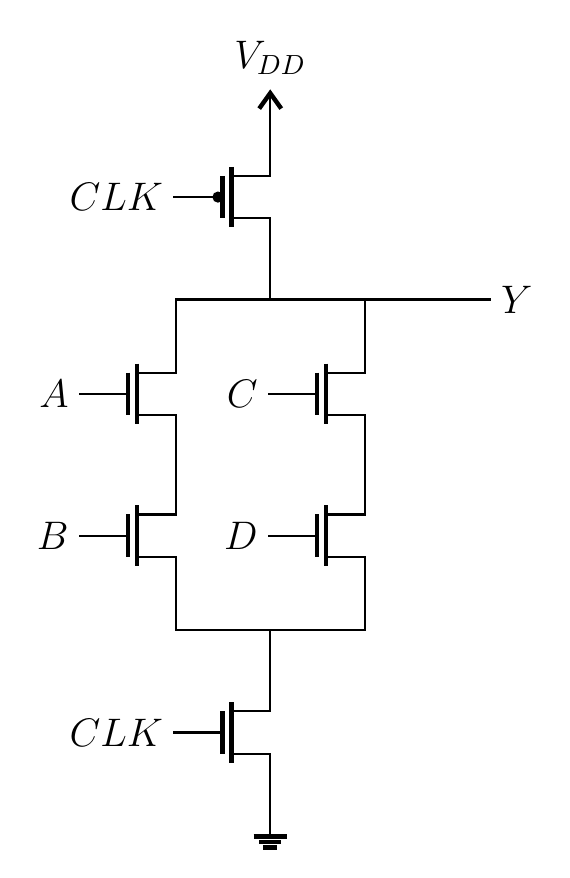
\begin{tikzpicture}[thick,font=\Large]\node[pmos](m55)at(0,1.3000000000000003){};\draw(0,2.2)--(m55.S)(m55.D)--(0,0.40000000000000013);\draw(m55.G)--++(-.25,0)node[left]{$CLK$};\draw(0,0)--(-1.2,0)--(-1.2,-0.3);\node[nmos](m56)at(-1.2,-1.2){};\draw(-1.2,-0.3)--(m56.D)(m56.S)--(-1.2,-2.1);\draw(m56.G)--++(-.25,0)node[left]{$A$};\node[nmos](m57)at(-1.2,-3.0){};\draw(-1.2,-2.1)--(m57.D)(m57.S)--(-1.2,-3.9000000000000004);\draw(m57.G)--++(-.25,0)node[left]{$B$};\draw(-1.2,-3.9)--(-1.2,-4.2)--(0,-4.2);\draw(0,0)--(1.2,0)--(1.2,-0.3);\node[nmos](m58)at(1.2,-1.2){};\draw(1.2,-0.3)--(m58.D)(m58.S)--(1.2,-2.1);\draw(m58.G)--++(-.25,0)node[left]{$C$};\node[nmos](m59)at(1.2,-3.0){};\draw(1.2,-2.1)--(m59.D)(m59.S)--(1.2,-3.9000000000000004);\draw(m59.G)--++(-.25,0)node[left]{$D$};\draw(1.2,-3.9)--(1.2,-4.2)--(0,-4.2);\node[nmos](m60)at(0,-5.500000000000001){};\draw(0,-4.6000000000000005)--(m60.D)(m60.S)--(0,-6.4);\draw(m60.G)--++(-.25,0)node[left]{$CLK$};\draw(0,2.2)node[vcc]{$V_{DD}$};\draw(0,.4)--(0,0)--(2.8,0);\draw(0,-4.2)--(0,-4.6000000000000005);\draw(0,-6.4)node[ground]{};\node[right]at(2.8,0){$Y$};\end{tikzpicture}
\end{document}
